\newpage
\section{Resultados}

\subsection{Modulador FSK}

A partir do gerador de áudio do módulo MCA 8801, foi gerado uma onda quadrada, simulando dessa forma um trem de pulsos, do tipo NRZ (Non-Return-to-Zero). O sinal foi ajustado para uma frequência de $1 kHz$, tensão de $400 mV_p$ e ciclo ativo de $50 \%$.

\begin{figure}[H]
    \centering
    \caption{Menssagem a ser transmitida, com 400mVp e razão cíclica de 50\%.}
    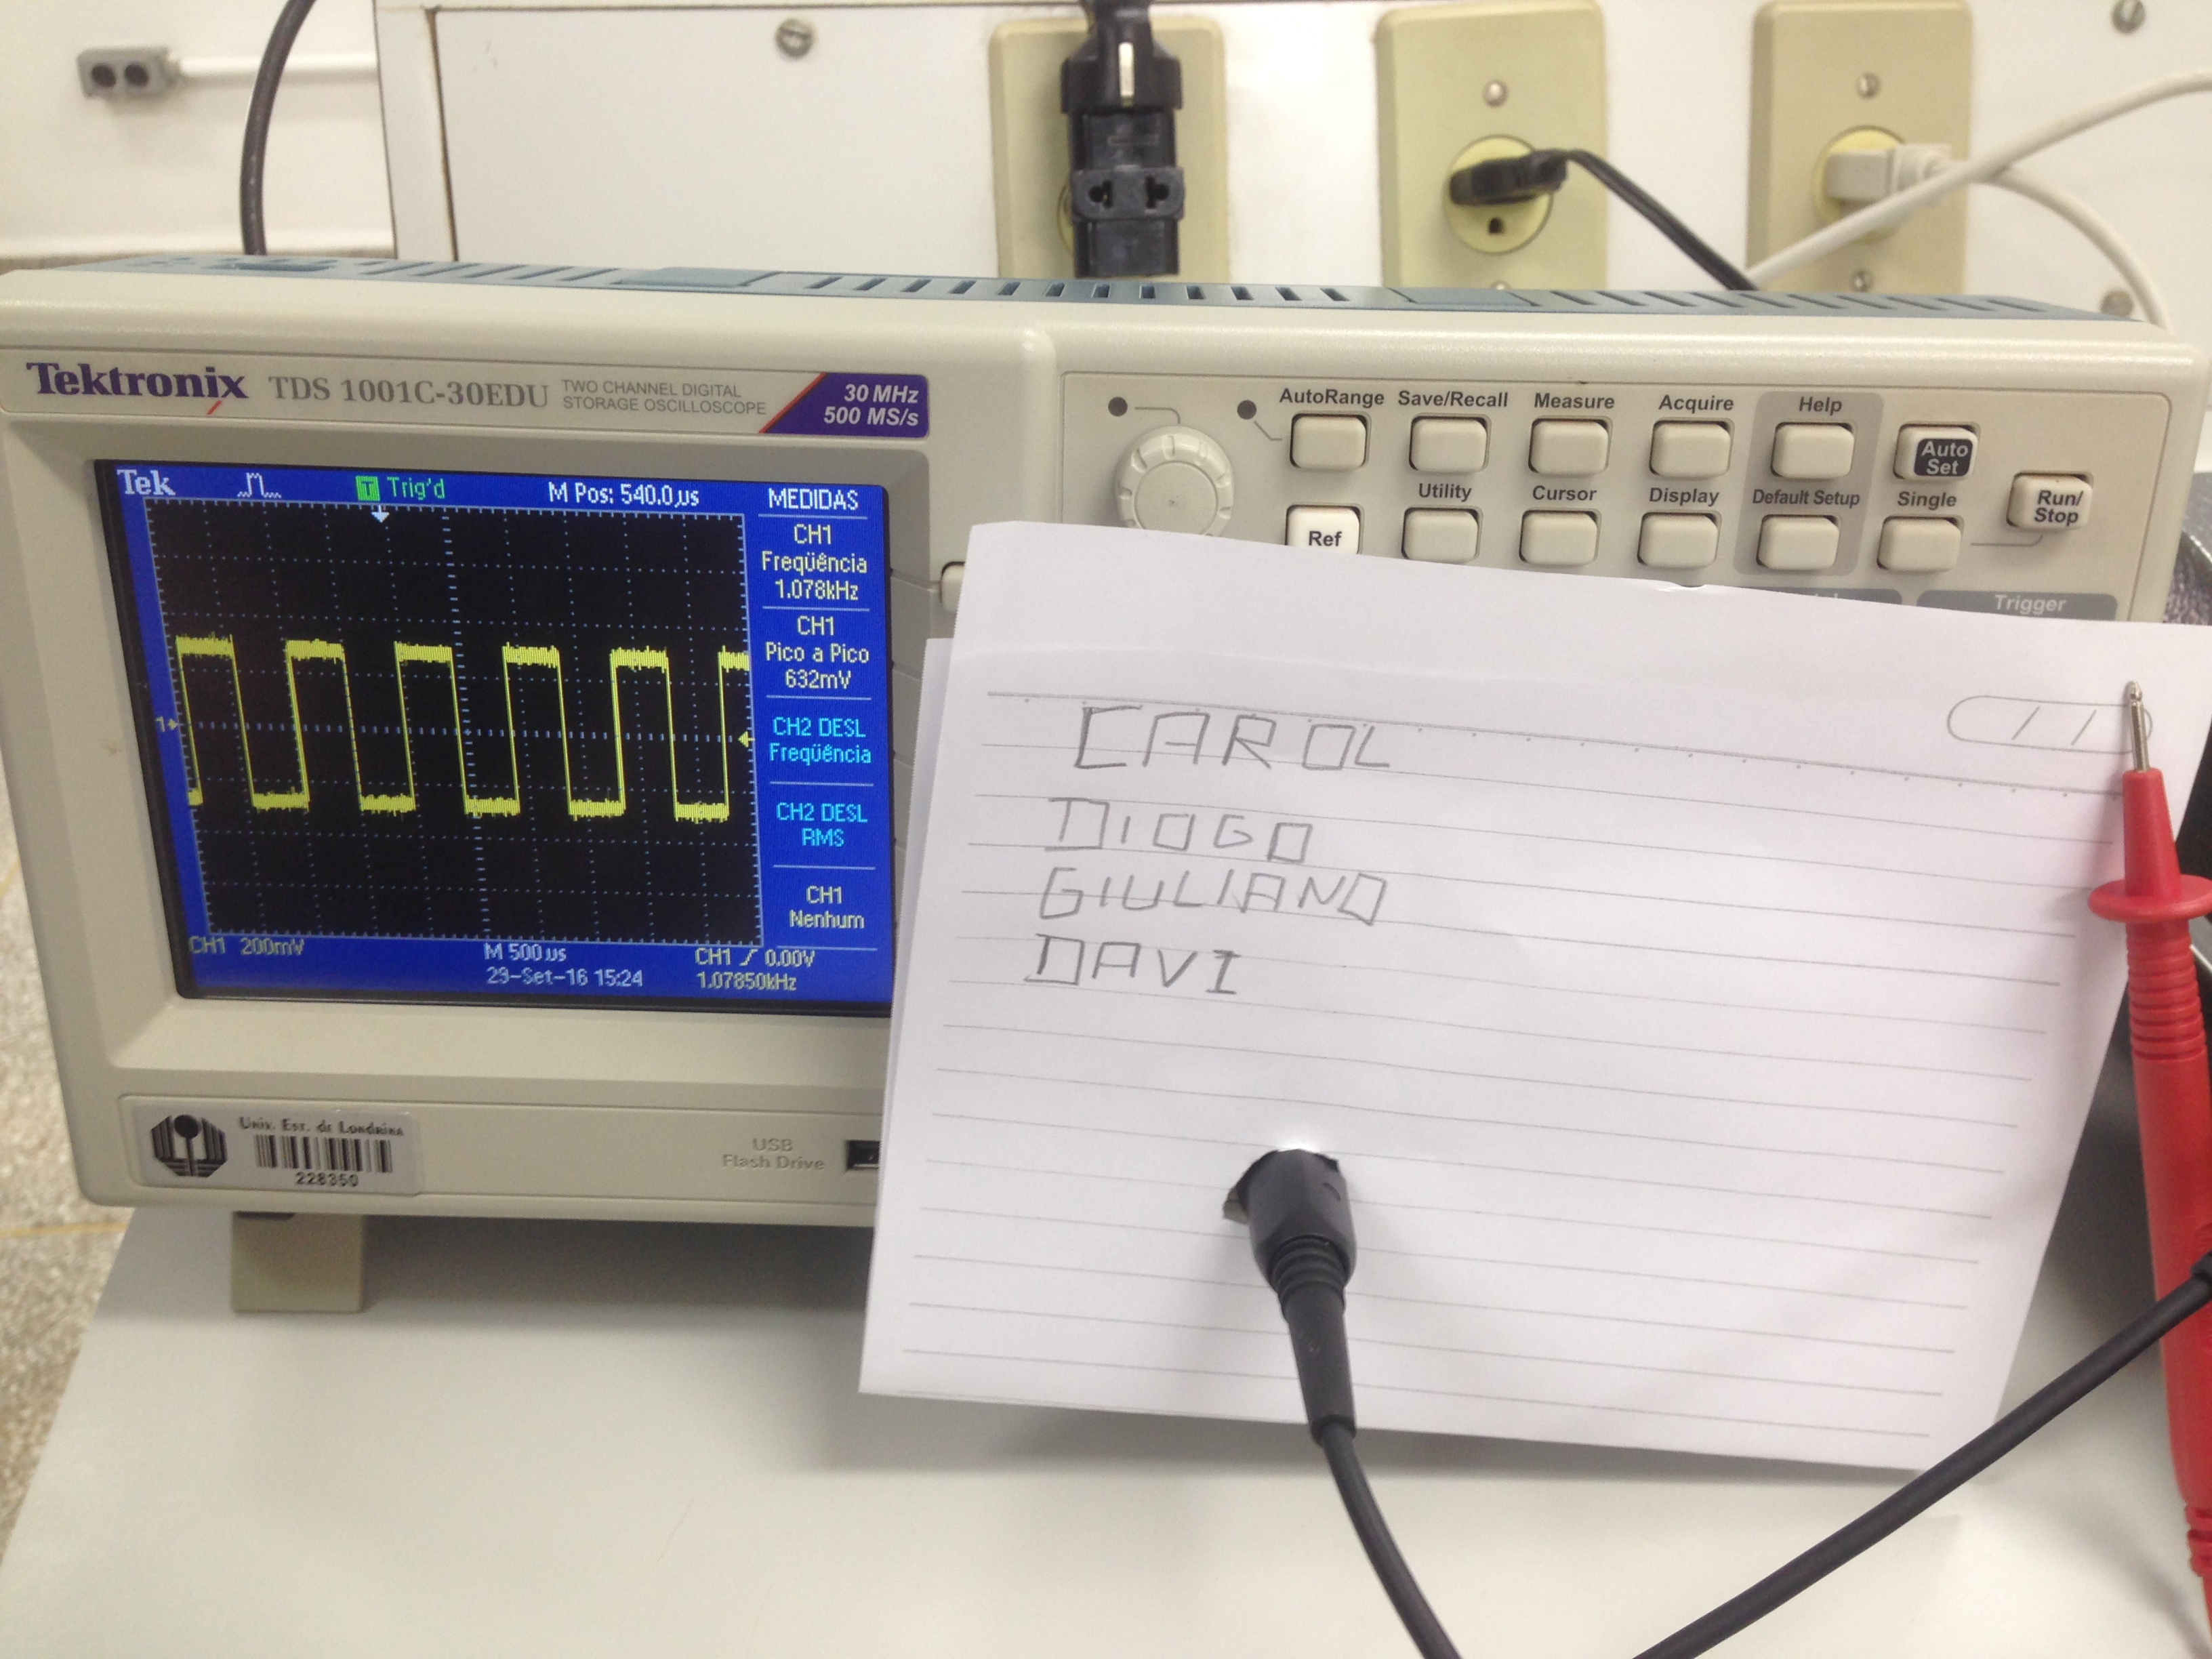
\includegraphics[scale=0.1]{m}
    \label{fig:m}
    
    \small Fonte: Autoria própria.
\end{figure}

Para ajusta a portadora do modulador FSK contido no módulo MCA 8801, foi ajustado, sem sinal de dados, uma frequência de $10 kHz$ a uma tensão de $1 V_p$. 

\begin{figure}[H]
    \centering
    \caption{Portadora para o modulador FSK.}
    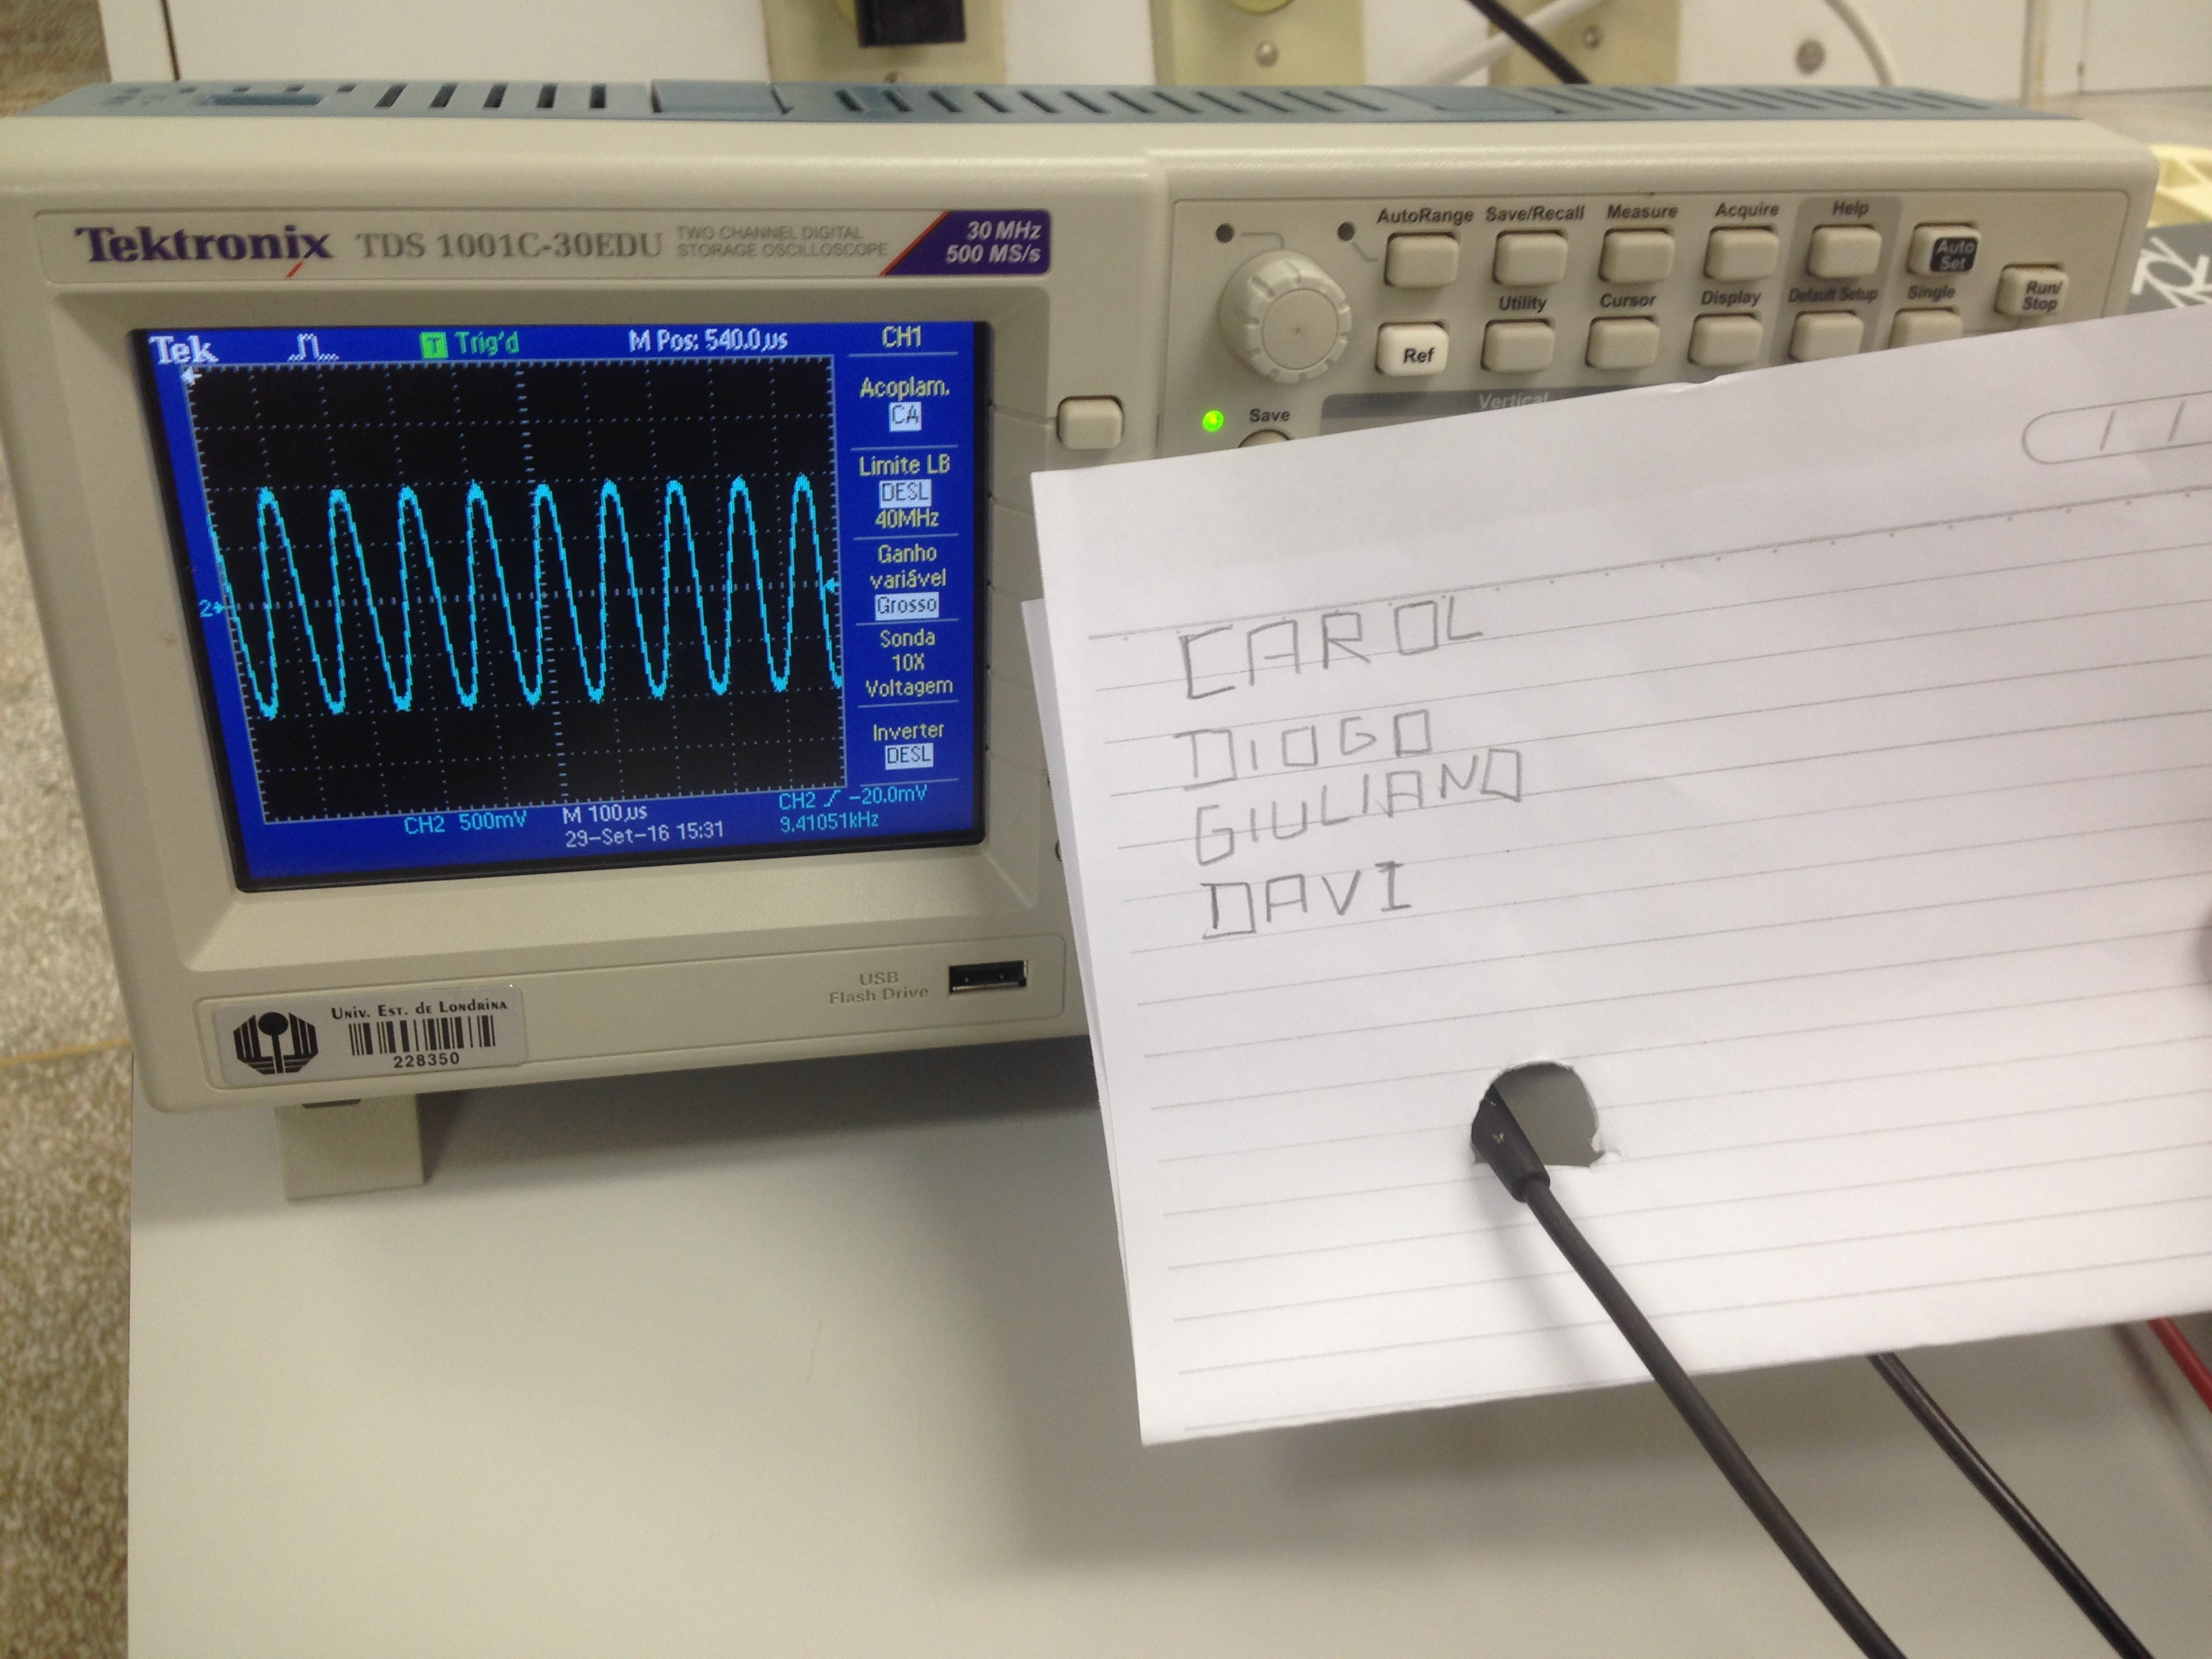
\includegraphics[scale=0.1]{c}
    \label{fig:c}
    
    \small Fonte: Autoria própria.
\end{figure}

Ajustado o sinal de dados e a portadora, os sinal de dados foi ligado no modulador, podendo assim obter os respectivos sinais mostrados na Figura \ref{fig:400}


\begin{figure}[H]
    \centering
    \caption{Saída modulada para entrada com 400mVp.}
    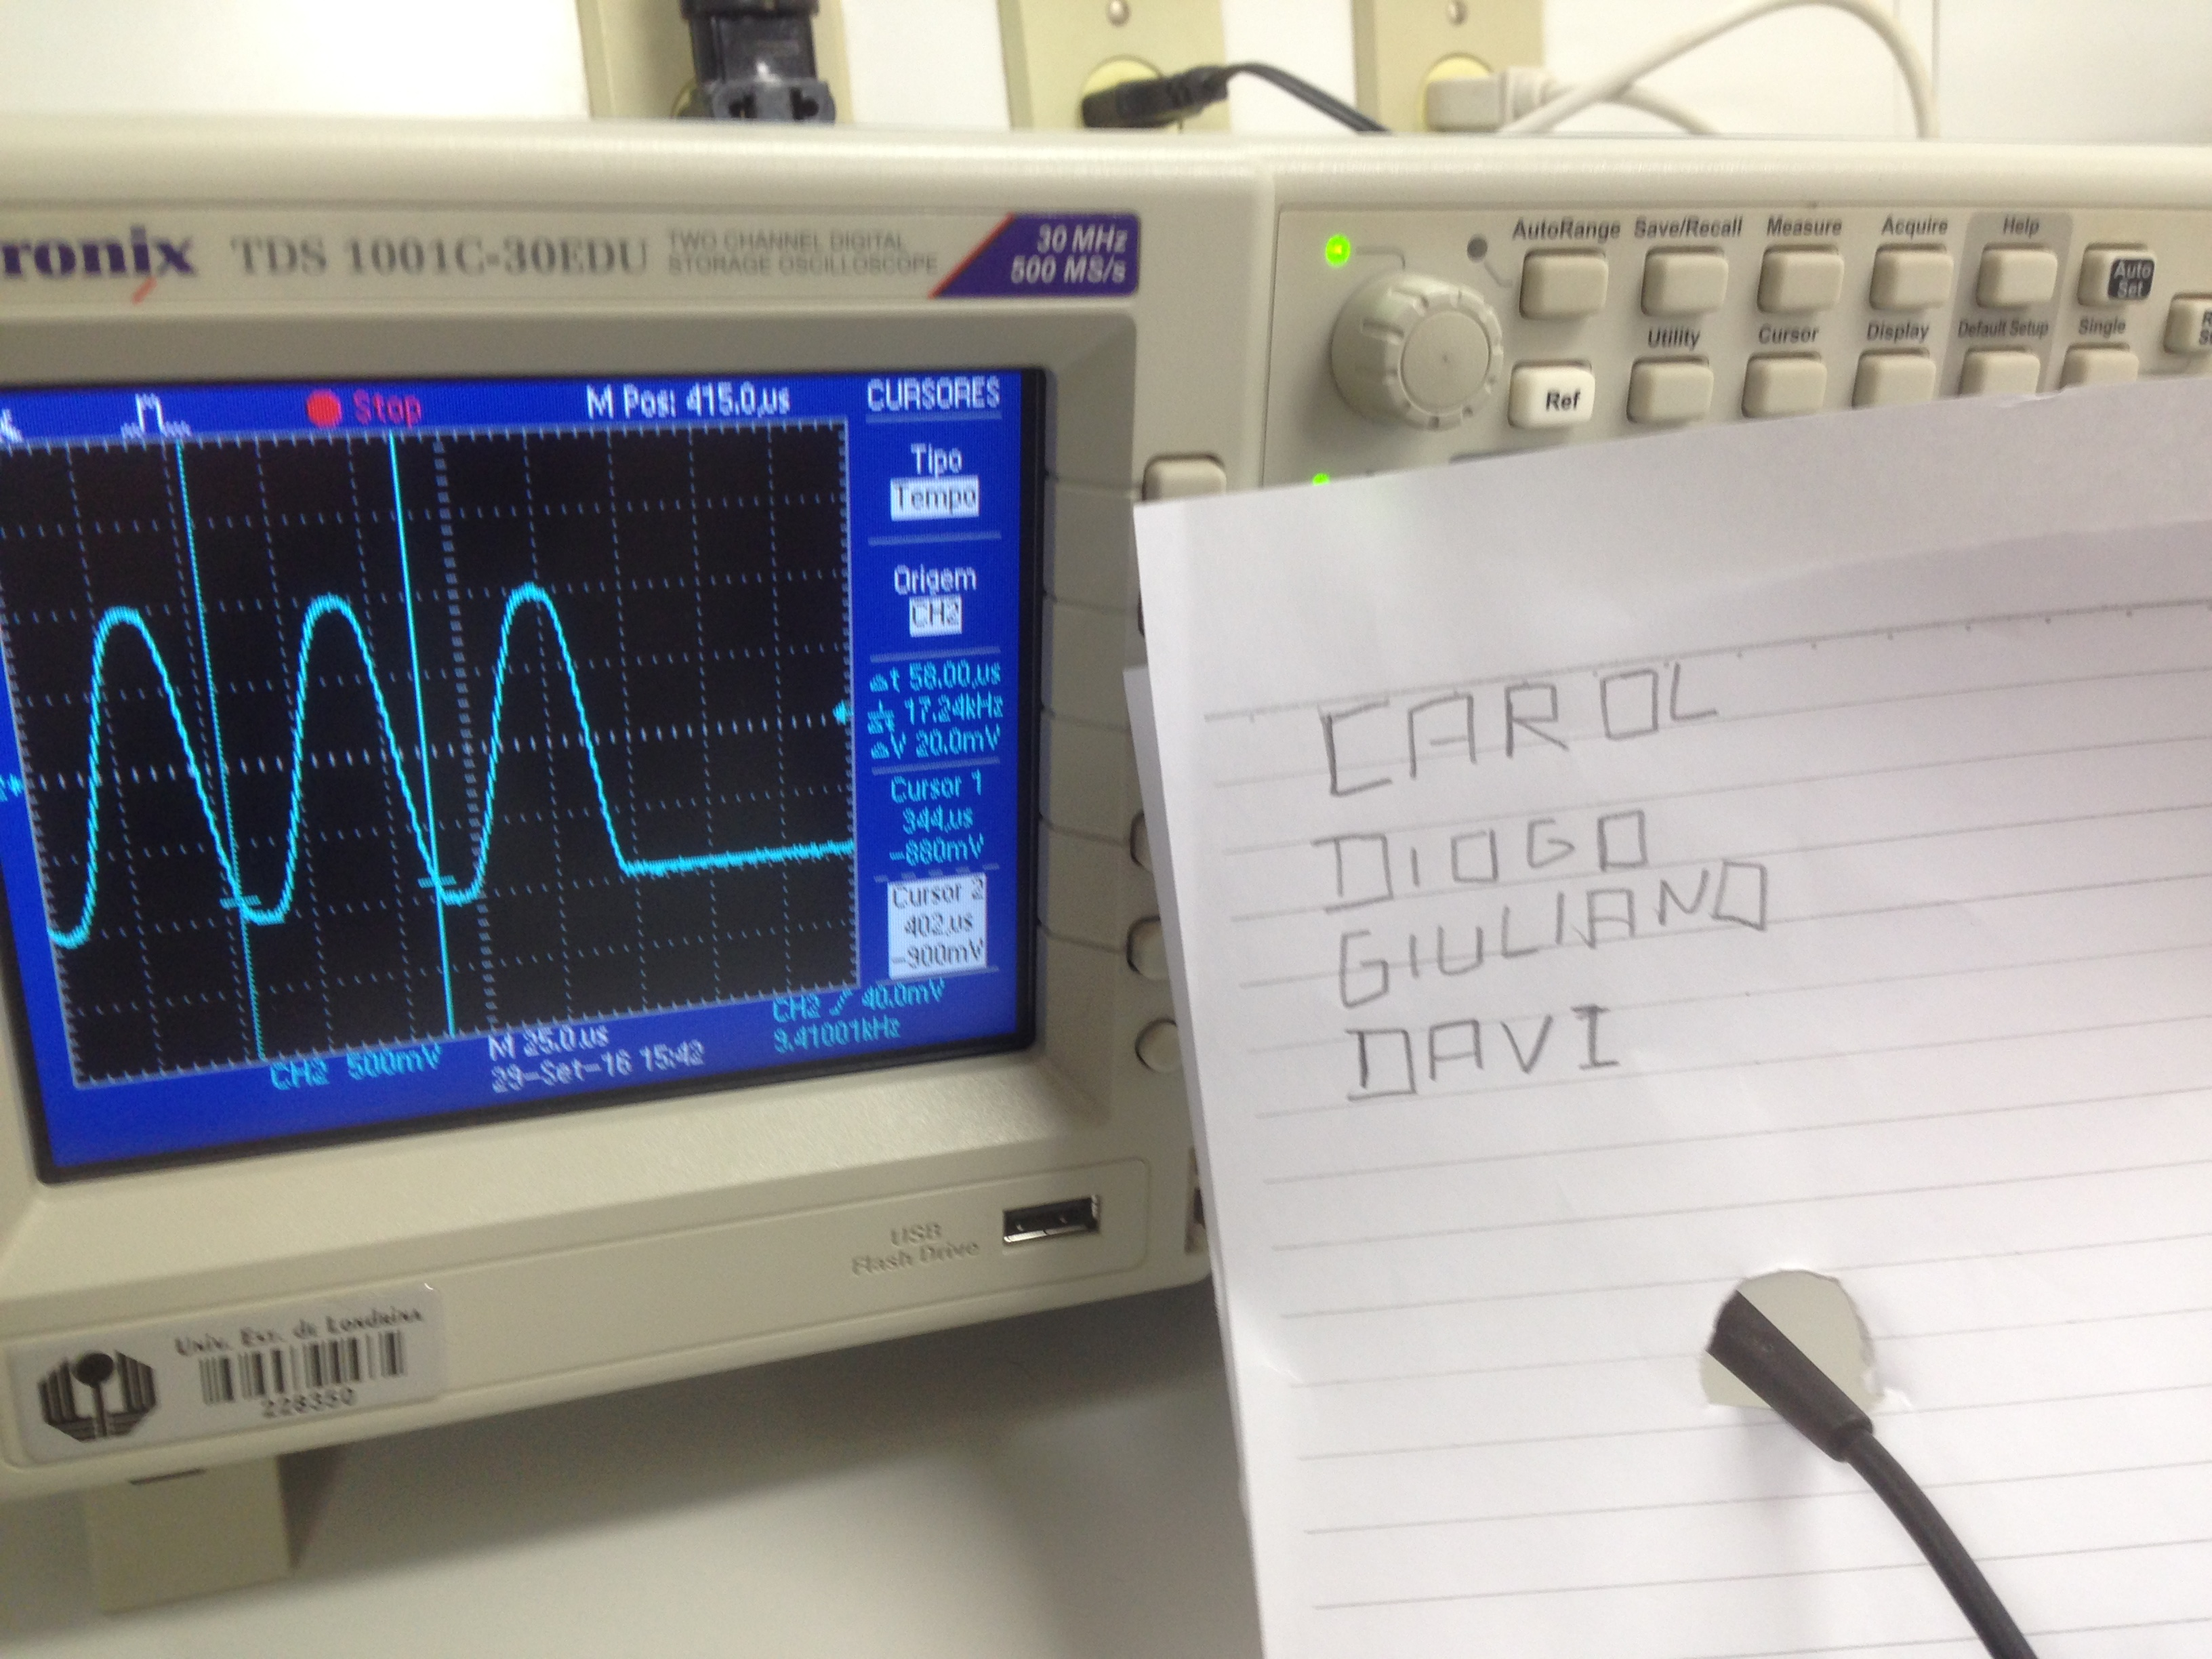
\includegraphics[scale=0.1]{400}
    \label{fig:400}
    
    \small Fonte:  Autoria própria.
\end{figure}

Nota-se que o sinal não corresponde a um BFSK, pois para a frequência mais baixa, $f_1$, não há senoide.

De forma a obter o deslocamento de frequência em resposta a onda quadrada, foi-se variando a amplitude do sinal de dados e, utilizando o cursor do osciloscópio, para obter as frequências $f_1$ e $f_2$. Os resultados foram montados na Tabela \ref{tab:400}.


\begin{table}[H]
    \centering
    \caption{Variação nas frequências de acordo com a tensão de entrada.}
    \begin{tabular}{|l|l|l|l|}
        \hline
        $V_p [mV]$ & $f_1 [kHz]$  & $f_2 [kHz]$ & $2 \Delta{f} [kHz]$ \\ 
        \hline
        400 & 17,8 & - & - \\ 
        \hline
        360 & 19,2 & - & - \\ 
        \hline
        320 & 19,2 & 2,8 & 16,4 \\ 
        \hline
        280 & 14,7 & 2,9 & 11,8 \\ 
        \hline
        240 & 14,7 & 3,2 & 11,5 \\ 
        \hline
        200 & 13,8 & 4,2 & 9,6 \\ 
        \hline
        160 & 13,1 & 5,6 & 7,4 \\ 
        \hline
        120 & 11,3 & 6,41 & 4,9 \\ 
        \hline
        80 & 11,1 & 7,69 & 3,4 \\ 
        \hline
        40 & 10,4 & 8,92 & 1,5 \\ 
        \hline
    \end{tabular}
\label{tab:400}

\small Fonte:  Autoria própria.
\end{table}


Observe na tabela, que somente existirá valor mensurável de $f_2$ quando $V_p \geq 320 mV$. Isso indica que o sinal só será FSK quando sua tensão de pico assumir valores menores que $320 mV$, caso contrário, é muito difícil verificar a forma de onda quando há um bit ‘0’.

De modo a determinar se existe linearidade entre tensão modulante e frequência modulada, foi gerada uma curva relacionando $V_p$ x $2 \Delta{f}$, vide Figura \ref{fig:df}.

\begin{figure}[H]
    \centering
    \caption{ $V_p$ x $2 \Delta{f}$.}
    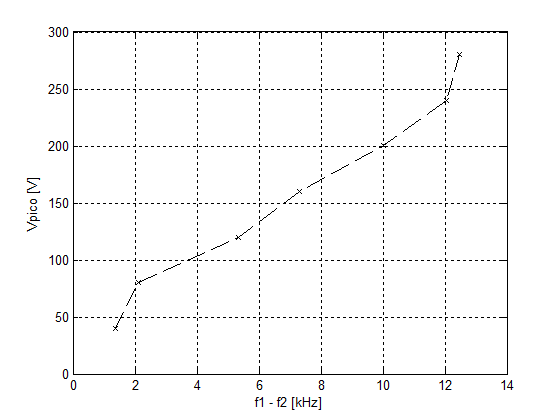
\includegraphics[scale=0.8]{curva}
    \label{fig:df}
    
    \small Fonte:  Autoria própria.
\end{figure}

Embora, a curva não seja puramente linear, podemos dizer que a relação é linear uma vez que devemos levar em consideração possíveis imprecisões e erros de medição e calibração. Mesmo assim, o resultado é bastante consistente. 

Durante o experimento, foi observada a descontinuidade de fase somente quando $2 \Delta{f}$ não é múltiplo da taxa de bit ($\frac{1}{T_b}$).

\subsection{Demodulador}

Para a demodulação do sinal modulado FSK, foi montado o circuito da Figura \ref{fig:montagem}, com base no CI 565 que corresponde a um PLL (Phase-Locked Loop).

\begin{figure}[H]
    \centering
    \caption{Circuito Demodulador FSK.}
    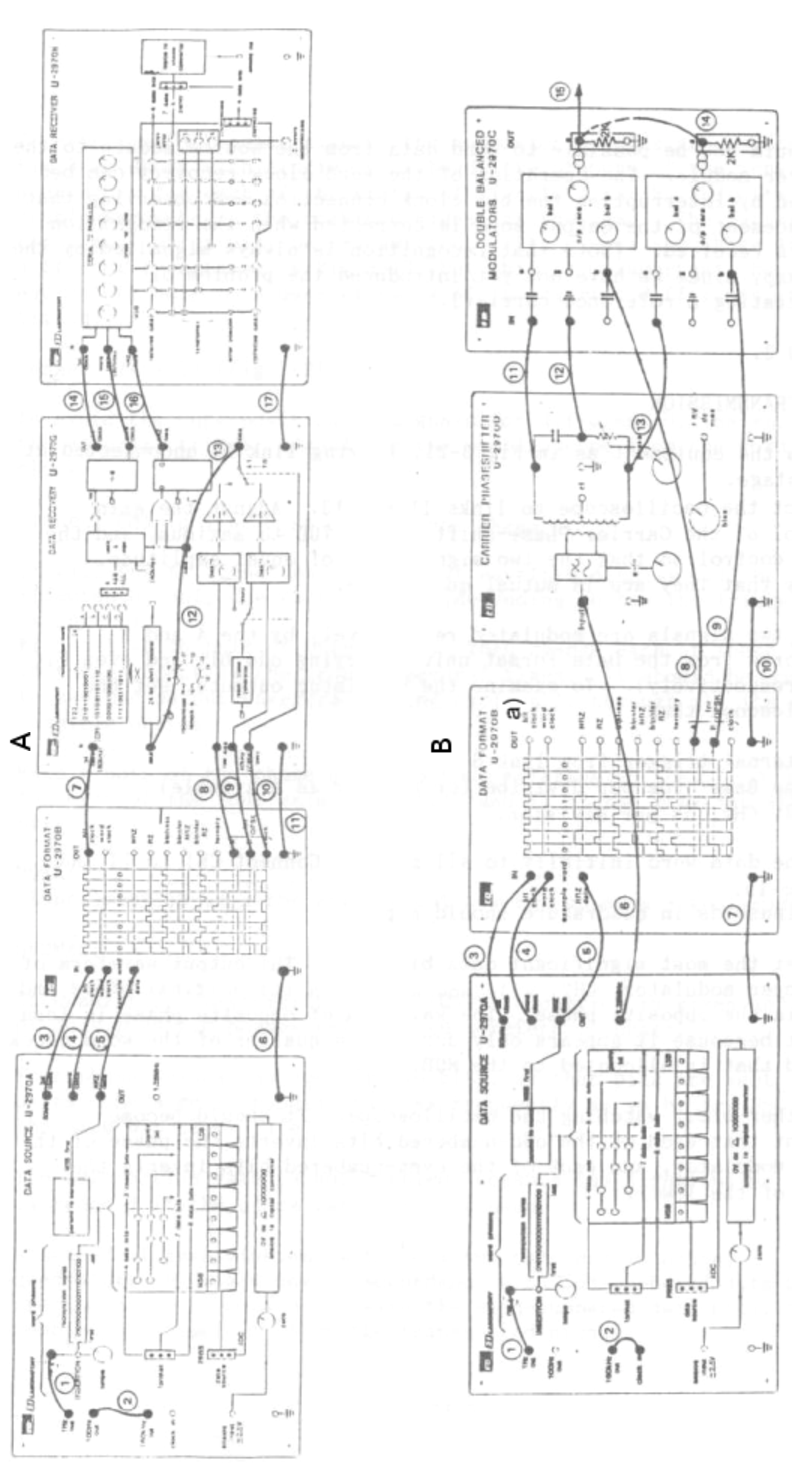
\includegraphics[scale=0.1]{montagem}
    \label{fig:montagem}
    
    \small Fonte:  Autoria própria.
\end{figure}

Conectado o modulador e com um ajuste fino em $R_{v1}$, foi possível recuperar o sinal modulante conforme a Figura \ref{fig:rec}.

\begin{figure}[H]
    \centering
    \caption{Sinal Modulante e Sinal Demodulado.}
    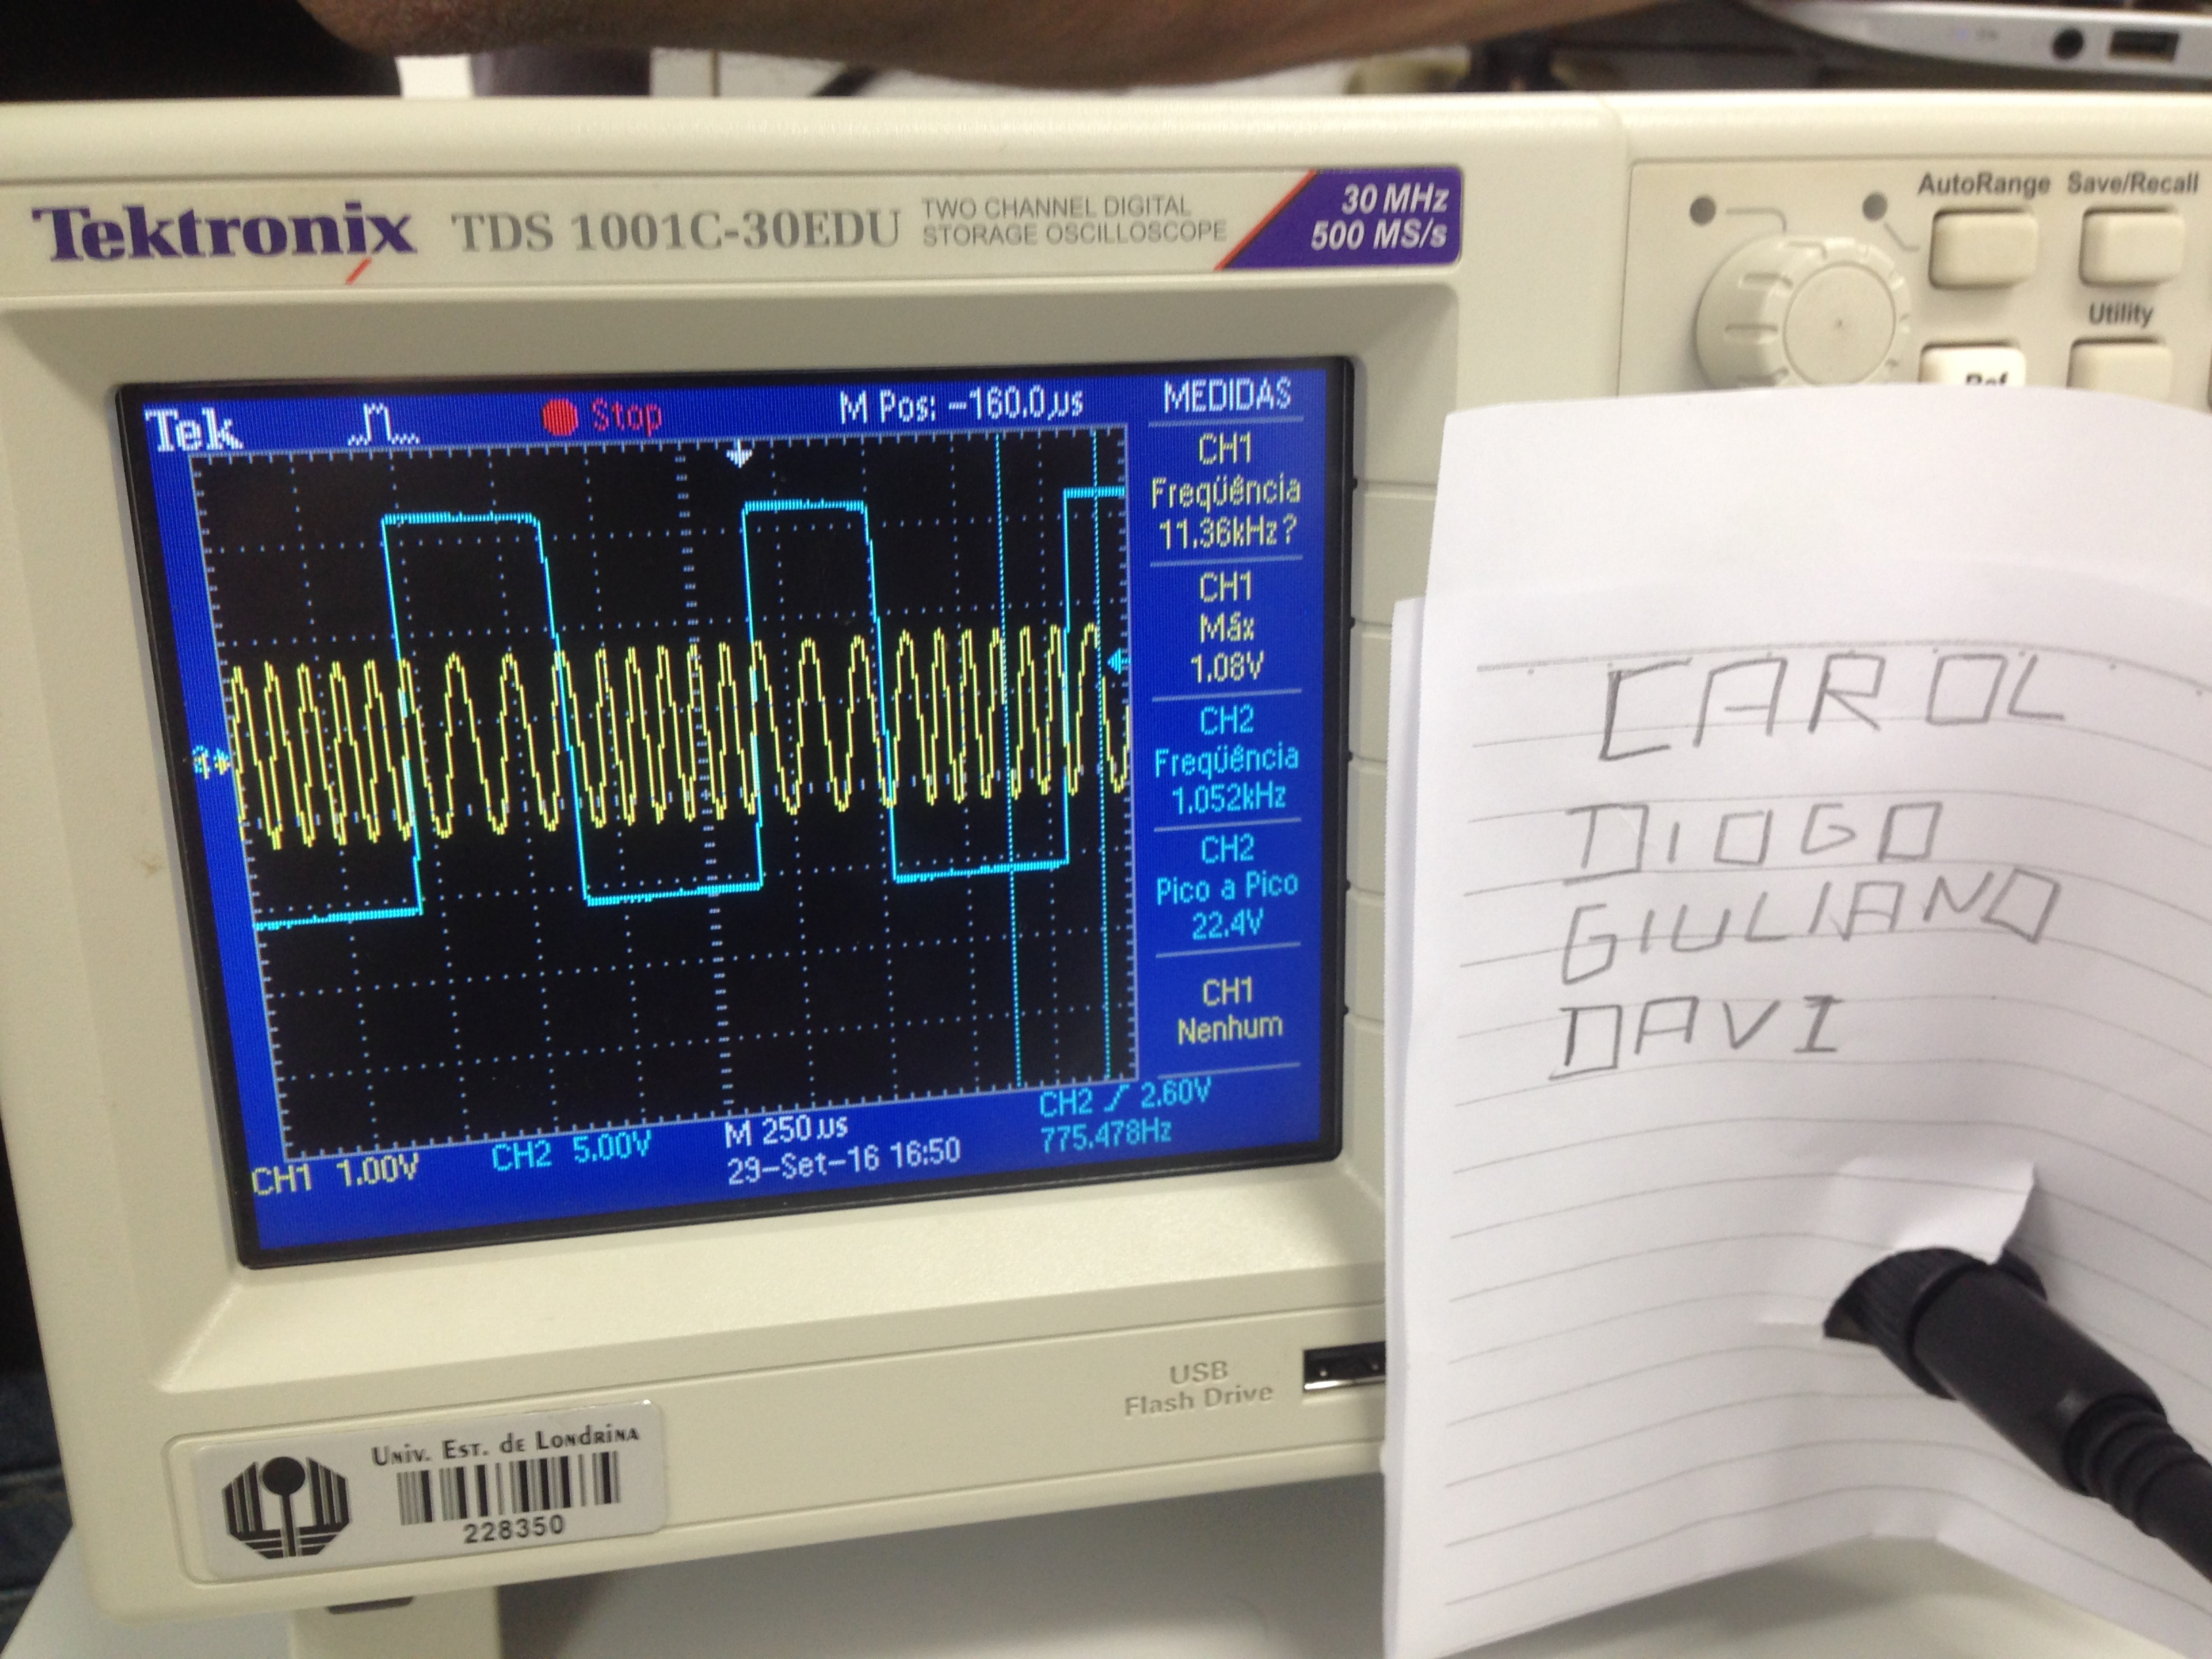
\includegraphics[scale=0.1]{rec}
    \label{fig:rec}
    
    \small Fonte:  Autoria própria.
\end{figure}

Ao desconectar a entrada de dados do modulador e posteriormente, conectar a entrada do modulador ao terra, foi realizada a medição da frequência correspondente a saída VCO (pino 4). Dessa forma, encontramos uma frequência VCO de $8,547 kHz$, conforme Figura \ref{fig:5}.

\begin{figure}[H]
    \centering
    \caption{Frequência VCO sem dados.}
    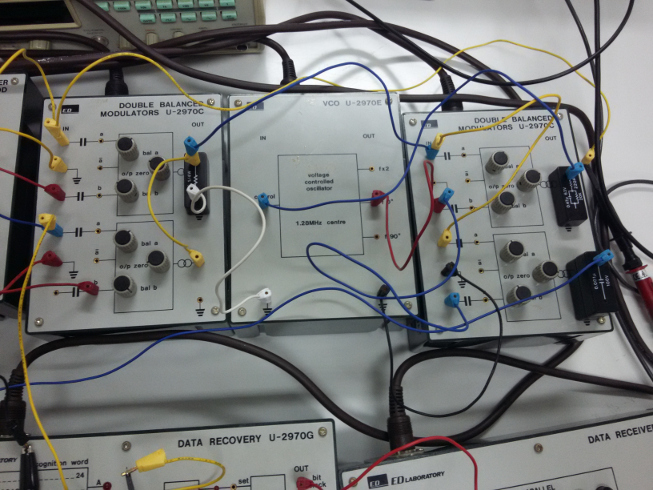
\includegraphics[scale=0.1]{5}
    \label{fig:5}
    
    \small Fonte:  Autoria própria.
\end{figure}

Reconectando a entrada de dados no modulador, podemos também verificar a frequência correspondente a saída VCO, conforme Figura \ref{fig:6}. Sendo assim, encontramos agora uma frequência de $11,63 kHz$.

\begin{figure}[H]
    \centering
    \caption{Frequência VCO com dados.}
    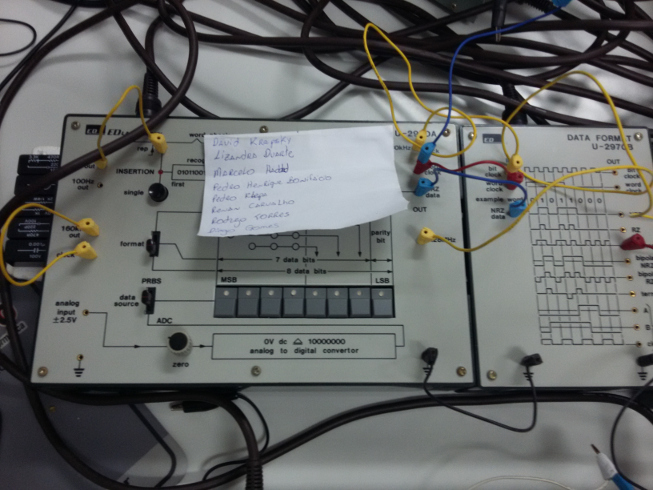
\includegraphics[scale=0.1]{6}
    \label{fig:6}
    
    \small Fonte:  Autoria própria.
\end{figure}

\newpage